% !TeX document-id = {4951685f-4d1a-4629-8de6-69a05c8522c0}
%  $Id: main.tex $
% !BIB TS-program = bibtex

\RequirePackage{graphicx}
\documentclass[10pt, conference, ]{IEEEtran}
\IEEEoverridecommandlockouts
% The preceding line is only needed to identify funding in the first footnote. If that is unneeded, please comment it out.
% $Id: preamble.tex 3335 2012-10-31 10:43:42Z nicolas.cardozo $

%----[ Packages ]---

\usepackage{ifdraft}

\usepackage[T1]{fontenc}
\usepackage[utf8]{inputenc}
\usepackage{amsmath}
\usepackage{mathrsfs}
\usepackage{hyperref}
\usepackage{wasysym}
%\usepackage{pxfonts}
\usepackage{yfonts}
\usepackage[plain]{fancyref}
\usepackage{subcaption}
\let\labelindent\relax
\usepackage[final]{listings}
\usepackage{booktabs}
\usepackage{multirow}
%\usepackage{threeparttable}
\usepackage{xcolor,colortbl}
\usepackage{xspace}
\usepackage{suffix}
\usepackage{etoolbox}
\usepackage[inline]{enumitem}
\usepackage{acronym}
\usepackage{url}

% Package 'biblatex'
\usepackage[backend=bibtex,
   style=ieee,
   citestyle=numeric-comp,
   natbib=true,
   maxnames=7,
   minnames=1,
   maxcitenames=1, 
   mincitenames=1,
   giveninits=true,
   hyperref=true,
   sorting=none,
   defernumbers]{biblatex}

%\renewcommand{\bibfont}{\footnotesize}

\addbibresource{bib/general.bib}
\addbibresource{bib/compsci.bib}
\addbibresource{bib/learning.bib}
\addbibresource{local.bib}

%\AtEveryBibitem{%
%   \clearlist{address}
%   \clearfield{date}
%   \clearfield{doi}
%   \clearfield{eprint}
%   \clearfield{isbn}
%   \clearfield{issn}
%   \clearfield{month}
%   \clearfield{note}
%   \clearfield{arxivId}
%   \clearfield{pages}
%   \clearfield{volume}
%   \clearfield{number}
%   \clearlist{location}
%   \clearfield{series}
%   \clearfield{url}
%   \clearname{editor}
%   \ifentrytype{inproceedings}
%     {\clearfield{day}
%      \clearfield{month}
%      \clearfield{volume}}{}
%}
%
%\DeclareFieldFormat*{title}{\textsl{#1}\isdot}
%\DeclareFieldFormat*{journaltitle}{#1}
%\DeclareFieldFormat*{booktitle}{#1}
%
%\renewcommand{\bibfont}{\footnotesize}
%\renewbibmacro{in:}{} % supress 'In: ' form
%\renewbibmacro{ser.}{} % supress 'ser.: ' form
%
%\DeclareSourcemap
% {\maps[datatype=bibtex,overwrite]
%   {% Tag entries (through keywords)
%    \map
%      {\step[fieldsource=publisher,
%       match=\regexp{Association for Computing Machinery}, replace={ACM}]}
%    \map
%      {\step[fieldsource=booktitle,
%       match=\regexp{[Pp]roceedings}, replace={Proc.}]}
%    \map
%      {\step[fieldsource=booktitle,
%       match=\regexp{[Ii]nternational}, replace={Intl.}]}
%    \map
%      {\step[fieldsource=booktitle,
%       match=\regexp{[Cc]onference}, replace={Conf.}]}
%    \map
%      {\step[fieldsource=booktitle,
%       match=\regexp{[Ff]oundation[s]}, replace={Found.}]}
%    \map
%      {\step[fieldsource=booktitle,
%       match=\regexp{[Ss]oftware}, replace={Soft.}]}
%    \map
%      {\step[fieldsource=booktitle,
%       match=\regexp{[Ee]ngineering}, replace={Eng.}]}
%    \map
%      {\step[fieldsource=booktitle,
%       match=\regexp{[Ss]ymposium}, replace={Symp.}]}
%    \map
%      {\step[fieldsource=journal,
%       match=\regexp{[Jj]ournal}, replace={Jour.}]}
%    \map
%      {\step[fieldsource=journal,
%       match=\regexp{[Ii]nternational}, replace={Intl.}]}
%    \map
%      {\step[fieldsource=journal,
%       match=\regexp{[Aa]pplications}, replace={Apps.}]}
%    \map
%      {\step[fieldsource=journal,
%       match=\regexp{[Ss]ystems}, replace={Sys.}]}
%    \map
%      {\step[fieldsource=journal,
%       match=\regexp{[Tt]ransactions}, replace={Trans.}]}
%    \map
%      {\step[fieldsource=journal,
%       match=\regexp{[Aa]utonomous and Adaptive Systems}, replace={Auton. Adapt. Syst.}]}
%    \map
%      {\step[fieldsource=booktitle,
%       match=\regexp{[Pp]roceedings\s+of\s+the.+[Ee]uropean\s+[Cc]onference\s+in}, replace={European Conf. in}]}
%    \map
%      {\step[fieldsource=booktitle,
%       match=\regexp{In\s+[Pp]roceedings\s+of\s+the\s+[Ss]ymposium\s+on}, replace={Symp. on}]}
%     \map
%      {\step[fieldsource=publisher,
%       match=\regexp{[Aa]ssociation\s+for\s+[Cc]omputing\s+[Mm]achinery\s}, replace={ACM}]}
%     \map
%      {\step[fieldsource=booktitle,
%       match=\regexp{[Pp]roceedings\s+of\s+the\s+[Ii]nternational\s+[Cc]onference\s+on}, replace={Intl. Conf. on}]}
%    \map
%      {\step[fieldsource=booktitle,
%       match=\regexp{[Pp]roceedings\s+of\s+the\s+[Ii]nternational\s+[Ww]orkshop\s+on}, replace={Intl. Workshop on}]}}}


%\theoremstyle{plain}
%\newtheorem{theorem}{Theorem}
%\newtheorem{lemma}{Lemma}%[section]
%\newtheorem{cor}{Corollary}[theorem]
%\theoremstyle{definition}
%\newtheorem{definition}{Definition}
%\newtheorem{ex}{Example}

% Avoid italics in examples (it's awful to read)
%\let\origEx\ex
%\let\origendEx\endex
%\renewenvironment{ex}{\origEx\upshape}{\origendEx}


% fancyref
\def\fref{\Fref} % treat all \frefs as \Frefs
\renewcommand{\lstlistingname}{Snippet}
\newcommand*{\fancyreflstlabelprefix}{lst} % define lst delimiter
\newcommand*{\Freflstname}{\lstlistingname}
\newcommand*{\freflstname}{\lstlistingname}
\Frefformat{vario}{\fancyreflstlabelprefix}%
  {\Freflstname\fancyrefdefaultspacing#1#3}
\frefformat{vario}{\fancyreflstlabelprefix}%
  {\freflstname\fancyrefdefaultspacing#1#3}
\Frefformat{plain}{\fancyreflstlabelprefix}%
  {\Freflstname\fancyrefdefaultspacing#1}
\frefformat{plain}{\fancyreflstlabelprefix}%
  {\freflstname\fancyrefdefaultspacing#1}

\newcommand*{\fancyrefthmlabelprefix}{thm} % define thm delimiter
\newcommand*{\Frefthmname}{Theorem}%
\newcommand*{\frefthmname}{%
 \MakeLowercase{\Frefthmname}}%
\Frefformat{vario}{\fancyrefthmlabelprefix}%
  {\Frefthmname\fancyrefdefaultspacing#1#3}
\frefformat{vario}{\fancyrefthmlabelprefix}%
  {\frefthmname\fancyrefdefaultspacing#1#3}
\Frefformat{plain}{\fancyrefthmlabelprefix}%
  {\Frefthmname\fancyrefdefaultspacing#1}
\frefformat{plain}{\fancyrefthmlabelprefix}%
  {\frefthmname\fancyrefdefaultspacing#1}

\newcommand*{\fancyreflemlabelprefix}{lem} % define lem delimiter
\newcommand*{\Freflemname}{Lemma}%
\newcommand*{\freflemname}{%
 \MakeLowercase{\Freflemname}}%
\Frefformat{vario}{\fancyreflemlabelprefix}%
  {\Freflemname\fancyrefdefaultspacing#1#3}
\frefformat{vario}{\fancyreflemlabelprefix}%
  {\freflemname\fancyrefdefaultspacing#1#3}
\Frefformat{plain}{\fancyreflemlabelprefix}%
  {\Freflemname\fancyrefdefaultspacing#1}
\frefformat{plain}{\fancyreflemlabelprefix}%
  {\freflemname\fancyrefdefaultspacing#1}

\newcommand*{\fancyrefdeflabelprefix}{def} % define def delimiter
\newcommand*{\Frefdefname}{Definition}%
\newcommand*{\frefdefname}{%
 \MakeLowercase{\Frefdefname}}%
\Frefformat{vario}{\fancyrefdeflabelprefix}%
  {\Frefdefname\fancyrefdefaultspacing#1#3}
\frefformat{vario}{\fancyrefdeflabelprefix}%
  {\frefdefname\fancyrefdefaultspacing#1#3}
\Frefformat{plain}{\fancyrefdeflabelprefix}%
  {\Frefdefname\fancyrefdefaultspacing#1}
\frefformat{plain}{\fancyrefdeflabelprefix}%
  {\frefdefname\fancyrefdefaultspacing#1}

\newcommand*{\fancyreflnlabelprefix}{ln} % define ln delimiter
\newcommand*{\Freflnname}{Line}%
\newcommand*{\freflnname}{%
 \MakeLowercase{\Freflnname}}%
\Frefformat{vario}{\fancyreflnlabelprefix}%
  {\Freflnname\fancyrefdefaultspacing#1#3}
\frefformat{vario}{\fancyreflnlabelprefix}%
  {\freflnname\fancyrefdefaultspacing#1#3}
\Frefformat{plain}{\fancyreflnlabelprefix}%
  {\Freflnname\fancyrefdefaultspacing#1}
\frefformat{plain}{\fancyreflnlabelprefix}%
  {\freflnname\fancyrefdefaultspacing#1}

% listings

\lstset{%
  basicstyle=\footnotesize\ttfamily,
  aboveskip=0\baselineskip,
  belowskip=0\baselineskip,
  commentstyle=\scriptsize\itshape,
%  prebreak=\mbox{$\hookleftarrow$},
  breaklines,
  numberblanklines=false,
  numberstyle=\tiny\color{gray}, 
  numbersep=0pt,
  escapechar=`,  
  numberbychapter=false}
  
\lstdefinestyle{floating}
 {frame=lines,
  float=hptb,
  captionpos=b,
  abovecaptionskip=-0pt}

% context traits listings
\lstdefinestyle{py}
 {language=Python,
  showstringspaces=false,
  keywordstyle=\ttfamily\bfseries,
  tabsize=2,
  style=floating,
  belowskip=-0\baselineskip,
  aboveskip=-0\baselineskip,
  morekeywords={}
}

%context traits environment    
\lstnewenvironment{python}[1][]
 {\lstset{style=py,#1}}{}  

 % Context Traits in line source-code
\newcommand{\spy}[1]{\lstinline[style=py]{#1}}


%% Petri nets
\usepackage[version=0.96]{pgf}
\usepackage{tikz}
\usetikzlibrary{arrows, shapes, backgrounds}
\usetikzlibrary{decorations.pathreplacing}
\usetikzlibrary{shapes.misc}
\usetikzlibrary{petri}\tikzstyle{place}=[circle,thick,draw=black!75,minimum size=5mm]
\tikzstyle{iplace}=[circle,dashed,thick,draw=black!75,minimum size=5mm]
\tikzstyle{itransition}=[rectangle,draw,thick,fill=black,minimum size=1mm]
\tikzstyle{etransition}=[rectangle,draw,thick,minimum size=1mm]
\tikzstyle{ctransition}=[rectangle,draw,color=black!45,thick,fill=black!45,minimum size=1mm]

\tikzstyle{copn}=
 [node distance=1.3cm, >=stealth', bend angle=45, auto,
  font=\fontsize{8}{8}\selectfont]

  
%----[ Commands ]---


%Latins
\newcommand{\eg}{\emph{e.g.,}\xspace}
\newcommand{\ie}{\emph{i.e.,}\xspace}
\newcommand{\cf}{\emph{cf.}\xspace}

% Sets

\renewcommand{\emptyset}{\varnothing} % Redefine LaTeX version with AMS version



% Contexts
\newcommand{\ctx}[1]{\texttt{\textsc{#1}}}

% Petri nets

\newcommand{\petrinet}[5][]
  {\ensuremath{\mathopen{<}{#2}_{#1},{#3}_{#1},{#4}_{#1},{#5}_{#1}\mathclose{>}}}

% CoPNs

\newcommand{\copn}[7][]
  {\ensuremath{\mathopen{<}
      {#2}_{#1},{#3}_{#1},{#4}_{#1},{#5}_{#1},{#6}_{#1},{#7}_{#1}
      \mathclose{>}}}

\WithSuffix\newcommand\copn*[1][]{\copn[#1]{P}{T}{f}{f_\circ}{\rho}{m_0}}

\newcommand{\clause}[3]
  {\ensuremath{#1 in T: \ifblank{#2}{}{#2 \Rightarrow} #3}}

% Context dependency relations

\newcommand{\exclusion}[2]{\ctx{#1}$\square$\---$\square$\ctx{#2}}
\newcommand{\weakInclusion}[2]{\ctx{#1}--$\rhd$\ctx{#2}}
\newcommand{\strongInclusion}[2]{\ctx{#1}--$\blacktriangleright$\ctx{#2}}
\newcommand{\requirement}[2]{\ctx{#1}--$\LHD$\ctx{#2}}


%comments
% xcolor
\definecolor{author}{rgb}{.5, .5, .5}
\definecolor{comment}{rgb}{.1, .0, .9}
\definecolor{note}{rgb}{.9, .4, .0}
\definecolor{idea}{rgb}{.1, .7, .0}
\definecolor{missing}{rgb}{.9, .1, .0}
\definecolor{OliveGreen}{rgb}{0,0.6,0.3}



\newcommand{\authorcomment}[3][comment]
  {\ifdraft{\noindent
      \fbox{\footnotesize\textcolor{author}{\textsc{#2}}}
      \textcolor{#1}{\textsl{#3}}}{}}


%----[ Hyphenation ]---

\hyphenation
  {a-vail-a-bil-i-ty
   im-ple-men-ta-tion
   caus-al-ly
   con-struct
   par-a-digm
   pro-gra-mming}

\makeatother

\endinput


% $Id: acronyms.tex  $
% !TEX root = main.tex

\acrodef{AI}{Artificial Intelligence}
\acrodef{API}{Application Programming Interface}
\acrodef{AOP}{Aspect-oriented Programming}
\acrodef{CAS}{Collective Adaptive Systems}
\acrodef{CONRL}[ConRL]{Constructivist Reinforcement Learning}
\acrodef{DSL}{Domain-Specific Language}
\acrodef{DNN}{Deep Neural Networks}
\acrodef{DQN}{Deep Q-learning}
\acrodef{LOC}{Lines of Code}
\acrodef{ML}{Machine Learning}
\acrodef{MDP}{Markov Decision Process}
\acrodef{MNC}{Multiply-Nested Container}
\acrodef{OOP}{Object-Oriented Programming}
\acrodef{PCA}{Principal Component Analysis}
\acrodef{PDG}{Program Dependence Graph}
\acrodef{RL}{Reinforcement Learning}



%---[ Acronyms Plurals Special Forms] ---


\newcommand{\acResetNonTrivial}
  {\acresetall
   \acused{CPU}
   \acused{API}
   \acused{LAN}
   \acused{SMT}
   \acused{GUI}}

\acResetNonTrivial


\endinput


\begin{document}

\title{Adapting the Behavior of Reinforcement Learning Agents to Changing Action Spaces and Reward Functions}

%\author{
%\IEEEauthorblockN{Raul de la Rosa}
%\IEEEauthorblockA{%\textit{ Department of Computer Science and Technology} \\
%\textit{Universidad de los Andes}\\
%Bogot\'a, Colombia \\
%c.delarosap@uniandes.edu.co}
%\and
%\IEEEauthorblockN{Ivana Dusparic}
%\IEEEauthorblockA{%\textit{School of Computer Science and Statistics} \\
%\textit{Trinity College Dublin}\\
%Dublin, Ireland \\
%ivana.dusparic@tcd.ie}
%\and
%\IEEEauthorblockN{Nicol\'as Cardozo}
%\IEEEauthorblockA{%\textit{Systems and Computing Engineering Department}\\
%\textit{Universidad de los Andes}\\
%Bogot\'a, Colombia \\
%n.cardozo@uniandes.edu.co}
%}
\author{
\IEEEauthorblockN{Author template}
\IEEEauthorblockA{%\textit{ Department of Computer Science and Technology} \\
\textit{University}\\
City, Country \\
university-email}
}

\maketitle




\begin{abstract}
In Reinforcement Learning, agents learn to solve specific tasks through the 
exploration of the environment in which they execute. Agents' behavior is
specialized towards a goal, gathered from the environment, according to the 
agent's actions. While effective in optimizing the behavior for a task, the 
performance of Agent's rapidly decreases when the initial conditions change.
This paper introduces \adaptiverl, a self-adaptive Q-learning agent that enables on-the-fly adaptation without full retraining. \adaptiverl leverages proactive environment monitoring and concept-drift detection to trigger dynamic adjustment of learning and exploration parameters only when needed, while preserving prior policy knowledge to mitigate catastrophic forgetting. Additionally, \adaptiverl supports seamless incorporation of new actions into the agent’s action space. We validate our approach on a standard RL benchmark with shifting reward functions and in a realistic traffic signal control application in a city grid, demonstrating superior convergence speed, resource efficiency, and continuous adaptation to evolving conditions.
\end{abstract}



\begin{IEEEkeywords}
Reinforcement Learning,  
Continual Reinforcement Learning,  
Q-learning,  
Concept Drift Detection,  
Adaptive Systems,  
Traffic Signal Control
\end{IEEEkeywords}

% $Id: introduction.tex $
% !TEX root = main.tex

\section{Introduction}
\label{sec:introduction}

\acf{RL} is a subset of \ac{ML} techniques in which agents learn by interacting with an environment, 
through trial and error. An agent receives a scalar reward (positive or negative) for each interaction 
step, based on the action taken. The objective of the agent is to maximize its cumulative long-term 
reward~\cite{sutton98}. Traditional \ac{RL} algorithms, such as Q-Learning, assume stationary 
\acp{MDP}, where transition probabilities and reward functions are constant over 
time~\cite{meta-rl-traffic}. However, this assumption restricts \ac{RL} agents' effectiveness in 
real-world environments, which often exhibit non-stationary characteristics like evolving state 
distributions, varying reward dynamics, and changing action 
spaces~\cite{khetarpal2022continualreinforcementlearningreview}.

To overcome these limitations, our work adopts a \acf{CRL} paradigm, where agents continuously 
adapt to environmental changes~\cite{abel2023definitioncontinualreinforcementlearning}. Approaches 
such as meta-learning~\cite{zintgraf21} and transfer learning~\cite{zhuang20} have shown promise 
within \ac{CRL}. Meta-learning allows an agent to \emph{learn how to learn}, enhancing adaptability in 
new contexts~\cite{beck2024surveymetareinforcementlearning}. Transfer learning leverages prior 
knowledge to accelerate learning in related tasks~\cite{chen2022transferredqlearning}.

This paper introduces \adaptiverl, a Q-learning-based \ac{RL} algorithm that incorporates adaptive 
mechanisms inspired by \ac{CRL} to account for environment changes in the goal/rewards definition 
or in the action space available to an agent. Our work is motivated by the suitability of \ac{RL} for 
self-adaptive systems, given its capacity to dynamically adjust behavior in response to environmental 
feedback~\cite{HENRICHS2022106940}. However, real-world scenarios such as traffic control 
present substantial challenges due to their inherent non-stationary dynamics~\cite{meta-rl-traffic}. 
We note, the problem of environment changes to the state space has been addressed~\cite{gueriau19}, 
while adaptations to the goals (\ie rewards) or action space remain an open question.

Our method effectively addresses non-stationary environments by continuously monitoring and 
updating agents' learning strategy. 

We validate \adaptiverl using a self-adaptive systems context, specifically applied to traffic signal 
control at city intersections. In our scenario signal phases continuously influence state transitions 
and rewards~\cite{meta-rl-traffic}. By demonstrating the effectiveness of \adaptiverl under these conditions, we underline its suitability for self-adaptive systems, particularly those relying on streaming data where concept drift may occur, making efficient adaptation essential.

%%possibly remove
This paper is structured as follows: \fref{sec:background} introduces theoretical foundations relevant to our implementation. \fref{sec:related} reviews related work. \fref{sec:implementation} presents the \adaptiverl algorithm. \fref{sec:validation} describes our validation approach in traffic signal control and discusses results. Finally, \fref{sec:conclusion} offers conclusions and future research directions.





\endinput


% $Id: conclusion.tex 
% !TEX root = main.tex

%%
\section{Background}
\label{sec:background}

%%%%
\subsection{\acl{RL}}

In \ac{RL}, intelligent agents learn to map environmental situations (environment states) to actions that maximize a numerical reward signal received from the environment over the long term~\cite{sutton18}. \ac{RL} problems are commonly formulated as Markov Decision Processes (MDPs), defined by the tuple $\mathcal{M} = \langle \mathcal{S}, \mathcal{A}, P, R, \gamma \rangle$, where:
$\mathcal{S}$ is the state space, comprising all relevant states of the environment;
$\mathcal{A}$ is the action space, i.e., the set of all actions the agent can perform to affect the environment;
$P(s_{t+1} \mid s_t, a_t)$ is the transition probability from state {\color{purple}$s_t$} to {\color{purple}$s_{t+1}$} under action {\color{purple}$a_t$};
$R(s_t, a_t)$ is the reward function, providing the numerical signal ($r$) that encodes the positive or negative impact of taking action {\color{purple}$a_t$} in state {\color{purple}$s_t$} at each execution step $t$; and $\gamma \in [0, 1]$ is the discount factor, which determines the importance of future rewards.

In stationary settings, $P$ and $R$ remain fixed over time, and the agent’s objective is to learn a policy $\pi: \mathcal{S} \to \mathcal{A}$ that maximizes the expected discounted return. However, real-world environments often violate this stationarity assumption: transition dynamics and/or reward functions may shift due to evolving conditions. We model such scenarios as \emph{non-stationary} MDPs, represented by a sequence
\[
\{\mathcal{M}_t\}_{t=1}^\infty
\quad\text{with}\quad
\mathcal{M}_t = \bigl\langle \mathcal{S}, \mathcal{A}_t, P_t, R_t, \gamma \bigr\rangle,
\]
where $P_t$ and/or $R_t$ change at unknown time steps $t$ (``concept drifts''). In this work, we further consider the novel scenario where the agent's action space $\mathcal{A}$ may also change over time. Detecting and adapting to these drifts is central to \ac{CRL}~\cite{khetarpal2022continualreinforcementlearningreview,abel2023definitioncontinualreinforcementlearning}, which treats learning as an ongoing process across a continually changing sequence of tasks.

Q-learning~\cite{watkins92} is a widely used model-free approach in \ac{RL}. The long-term quality of an action performed at a given state is computed iteratively in a series of steps and is represented by a Q value,
$\mathit{Q(s,a)}$.
Formally, each execution step $t$ captures information from the environment and maps it to a state
{\color{purple}$s_t$} $\in \mathcal{S}$ in its state space. It then selects an
action {\color{purple}$a_t$} $\in \mathcal{A}$ from its action space and executes it. The agent
receives a reward {\color{Bittersweet}$r_t$} from the environment when it moves to the next state
$s_{t+1} \in \mathcal{S}$. The reward is used to update the optimality of performing the
action {\color{Mulberry}$a_t$} at state {\color{purple}$s_t$}. The agent's goal is to learn
a policy (\i.e. the best-fit action for each state) that maximizes the reward of the
long-run behavior. The learning rate \lrate{\alpha} determines how much new experiences 
overwrite previously learned experiences, and the discount factor {\color{RoyalBlue} $\gamma$} 
determines how much future rewards are discounted so that agents prioritize immediate actions and 
can plan the best long-term actions. At each time step $t$, the Q value of an action 
{\color{purple}$a_{t+1}$} taken in state {\color{purple}$s_{t+1}$}, $Q(s_{t+1}, a_{t+1})$, is updated by 
the Bellman learning equation as follows:

\vspace{1em}

\begin{equation*} \label{eq:QL}
     {\tikzmarknode{qt}{\highlight{purple}{$Q(s_t, a_t)$}}} +
    {\tikzmarknode{alpha}{\highlight{NavyBlue}{$\alpha$}}}
    [ 
    {\tikzmarknode{r}{\highlight{Bittersweet}{$r_{t+1}$}}}  +  
    {\tikzmarknode{gamma}{\highlight{RoyalBlue}{$\gamma$}}}
    {\tikzmarknode{max}{\highlight{OliveGreen}{$\max\limits_a Q(s_{t+1},a)$}}} - 
    {\tikzmarknode{qt2}{\highlight{purple}{$Q(s_t, a_t)$}}} 
    ]
\end{equation*}

\begin{tikzpicture}[overlay,remember picture,>=stealth,nodes={align=left,inner ysep=1pt},<-]
    % For "Qt1"
    \path (qt.north) ++ (3.9,1.7em) node[anchor=south east,color=Mulberry!85] (ntext){\textsf{\footnotesize Q-value}};
    \draw [color=Mulberry](qt.north) |- ([xshift=0.8ex,color=Mulberry]ntext.south west);
    \path (qt2.north) ++ (-2.2,1.8em) node[anchor=south east,color=Mulberry!85] (qt2text){};
    \draw [color=Mulberry](qt2.north) |- ([xshift=-4.9ex,color=Mulberry]qt2text.south west);
    % For alpha
    \path (alpha.north) ++ (-0.2,-2.8em) node[anchor=south east,color=NavyBlue] (atext){\textsf{\footnotesize learning rate}};
    \draw [color=NavyBlue](alpha.south) |- ([xshift=-9.3ex,color=NavyBlue]atext.south east);
    % For r
    \path (r.north) ++ (-0.1,1.5em) node[anchor=north east,color=Bittersweet!85] (lijtext){\textsf{\footnotesize reward}};
    \draw [color=Bittersweet](r.north) |- ([xshift=-4.3ex,color=Bittersweet]lijtext.south east);
    %gamma
    \path (gamma.north) ++ (0.5,1.5em) node[anchor=north west,color=RoyalBlue!85] (gtext){\textsf{\footnotesize discount factor}};
    \draw [color=RoyalBlue](gamma.north) |- ([xshift=-2.9ex,color=RoyalBlue]gtext.south east);
    % For "l_i^max"
    \path (max.north) ++ (-1.2,-3.6em) node[anchor=south west,color=xkcdHunterGreen!85] (lmaxtext){\textsf{\scriptsize Maximum Q-Value in the next state}};
    \draw [color=xkcdHunterGreen](max.south) |- ([xshift=-5ex,color=xkcdHunterGreen]lmaxtext.north);
\end{tikzpicture}




\endinput

\hfil

\begin{minipage}{0.5\columnwidth}
\begin{equation*}
    \label{eq:ab_crypto}
    \hspace*{-6em}
    X_{i} = \frac{1}{\sum_{i=1}^{\tikzmarknode{n}{\highlight{purple}{N}}} 
    \sum_{j=1}^{\tikzmarknode{mi}{\highlight{blue}{$M_i$}}} 
    \tfrac{\tikzmarknode{lij}{\highlight{Bittersweet}{$l_i^j$}}}{\tikzmarknode{lmax}{\highlight{OliveGreen}{$l^{max}$}}}
    }
\end{equation*}
\vspace*{0.8\baselineskip}
\begin{tikzpicture}[overlay,remember picture,>=stealth,nodes={align=left,inner ysep=1pt},<-]
    % For "N"
    \path (n.north) ++ (0,1.8em) node[anchor=south east,color=Plum!85] (ntext){\textsf{\footnotesize number of objects}};
    \draw [color=Plum](n.north) |- ([xshift=-0.3ex,color=Plum]ntext.south west);
    % For "M_i"
    \path (mi.north) ++ (0,3.5em) node[anchor=north west,color=blue!85] (mitext){\textsf{\footnotesize number of other objects}};
    \draw [color=blue](mi.north) |- ([xshift=-0.3ex,color=blue]mitext.south east);
    % For "l_i^j"
    \path (lij.north) ++ (0,1.9em) node[anchor=north west,color=Bittersweet!85] (lijtext){\textsf{\footnotesize size of j\textsuperscript{th} service}};
    \draw [color=Bittersweet](lij.north) |- ([xshift=-0.3ex,color=Bittersweet]lijtext.south east);
    % For "l_i^max"
    \path (lmax.north) ++ (-2.7,-1.5em) node[anchor=north west,color=xkcdHunterGreen!85] (lmaxtext){\textsf{\footnotesize maximum obj size}};
    \draw [color=xkcdHunterGreen](lmax.south) |- ([xshift=-0.3ex,color=xkcdHunterGreen]lmaxtext.south west);
\end{tikzpicture}
\end{minipage}
\caption{Two Equations side-by-side using minipage and figure constructs.}

While Q-learning converges under stationary conditions (with appropriate decay of \lrate{\alpha}), it can struggle when $P_t$ or $R_t$ change over time. Our work builds on this foundation by incorporating online concept-drift detection and adaptive updates, enabling the agent to remain effective in non-stationary MDPs. We focus particularly on shifts in $R_t$, which may also induce changes in $\mathcal{A}_t$.


%%%%
\subsection{Motivating example}
\label{sec:motivation}


To motivate the adaptation of agent's behavior to changing goals and the acquisition of new actions, 
we use the Gridworld benchmark as a running example.
Gridworld consists of a rectangular matrix ($9\times 9$ in our case). In Gridworld, every cell is 
associated with a reward of $-1$, except for a single goal state that has a reward of $+100$ as shown 
in the left part of \fref{fig:r-change}. The agent begins each episode at the grid's center and may move 
in any direction \spy{up}, \spy{down}, \spy{left}, or \spy{right}. Initially, the goal is placed in the top-left 
corner, but it may be relocated to any other position, as illustrated on the right-hand side of \fref{fig:r-change}. We also consider scenarios in which Gridworld contains walls that block the agent's movement according to its initial set of actions (see \fref{fig:q-value-comp2}). Subsequently, the action space is extended to include new actions that provide the agent with additional capabilities (e.g., jumping). The agent is expected to adapt to these changes and efficiently adjust its policy.

\begin{figure*}[hptb]
    \centering
    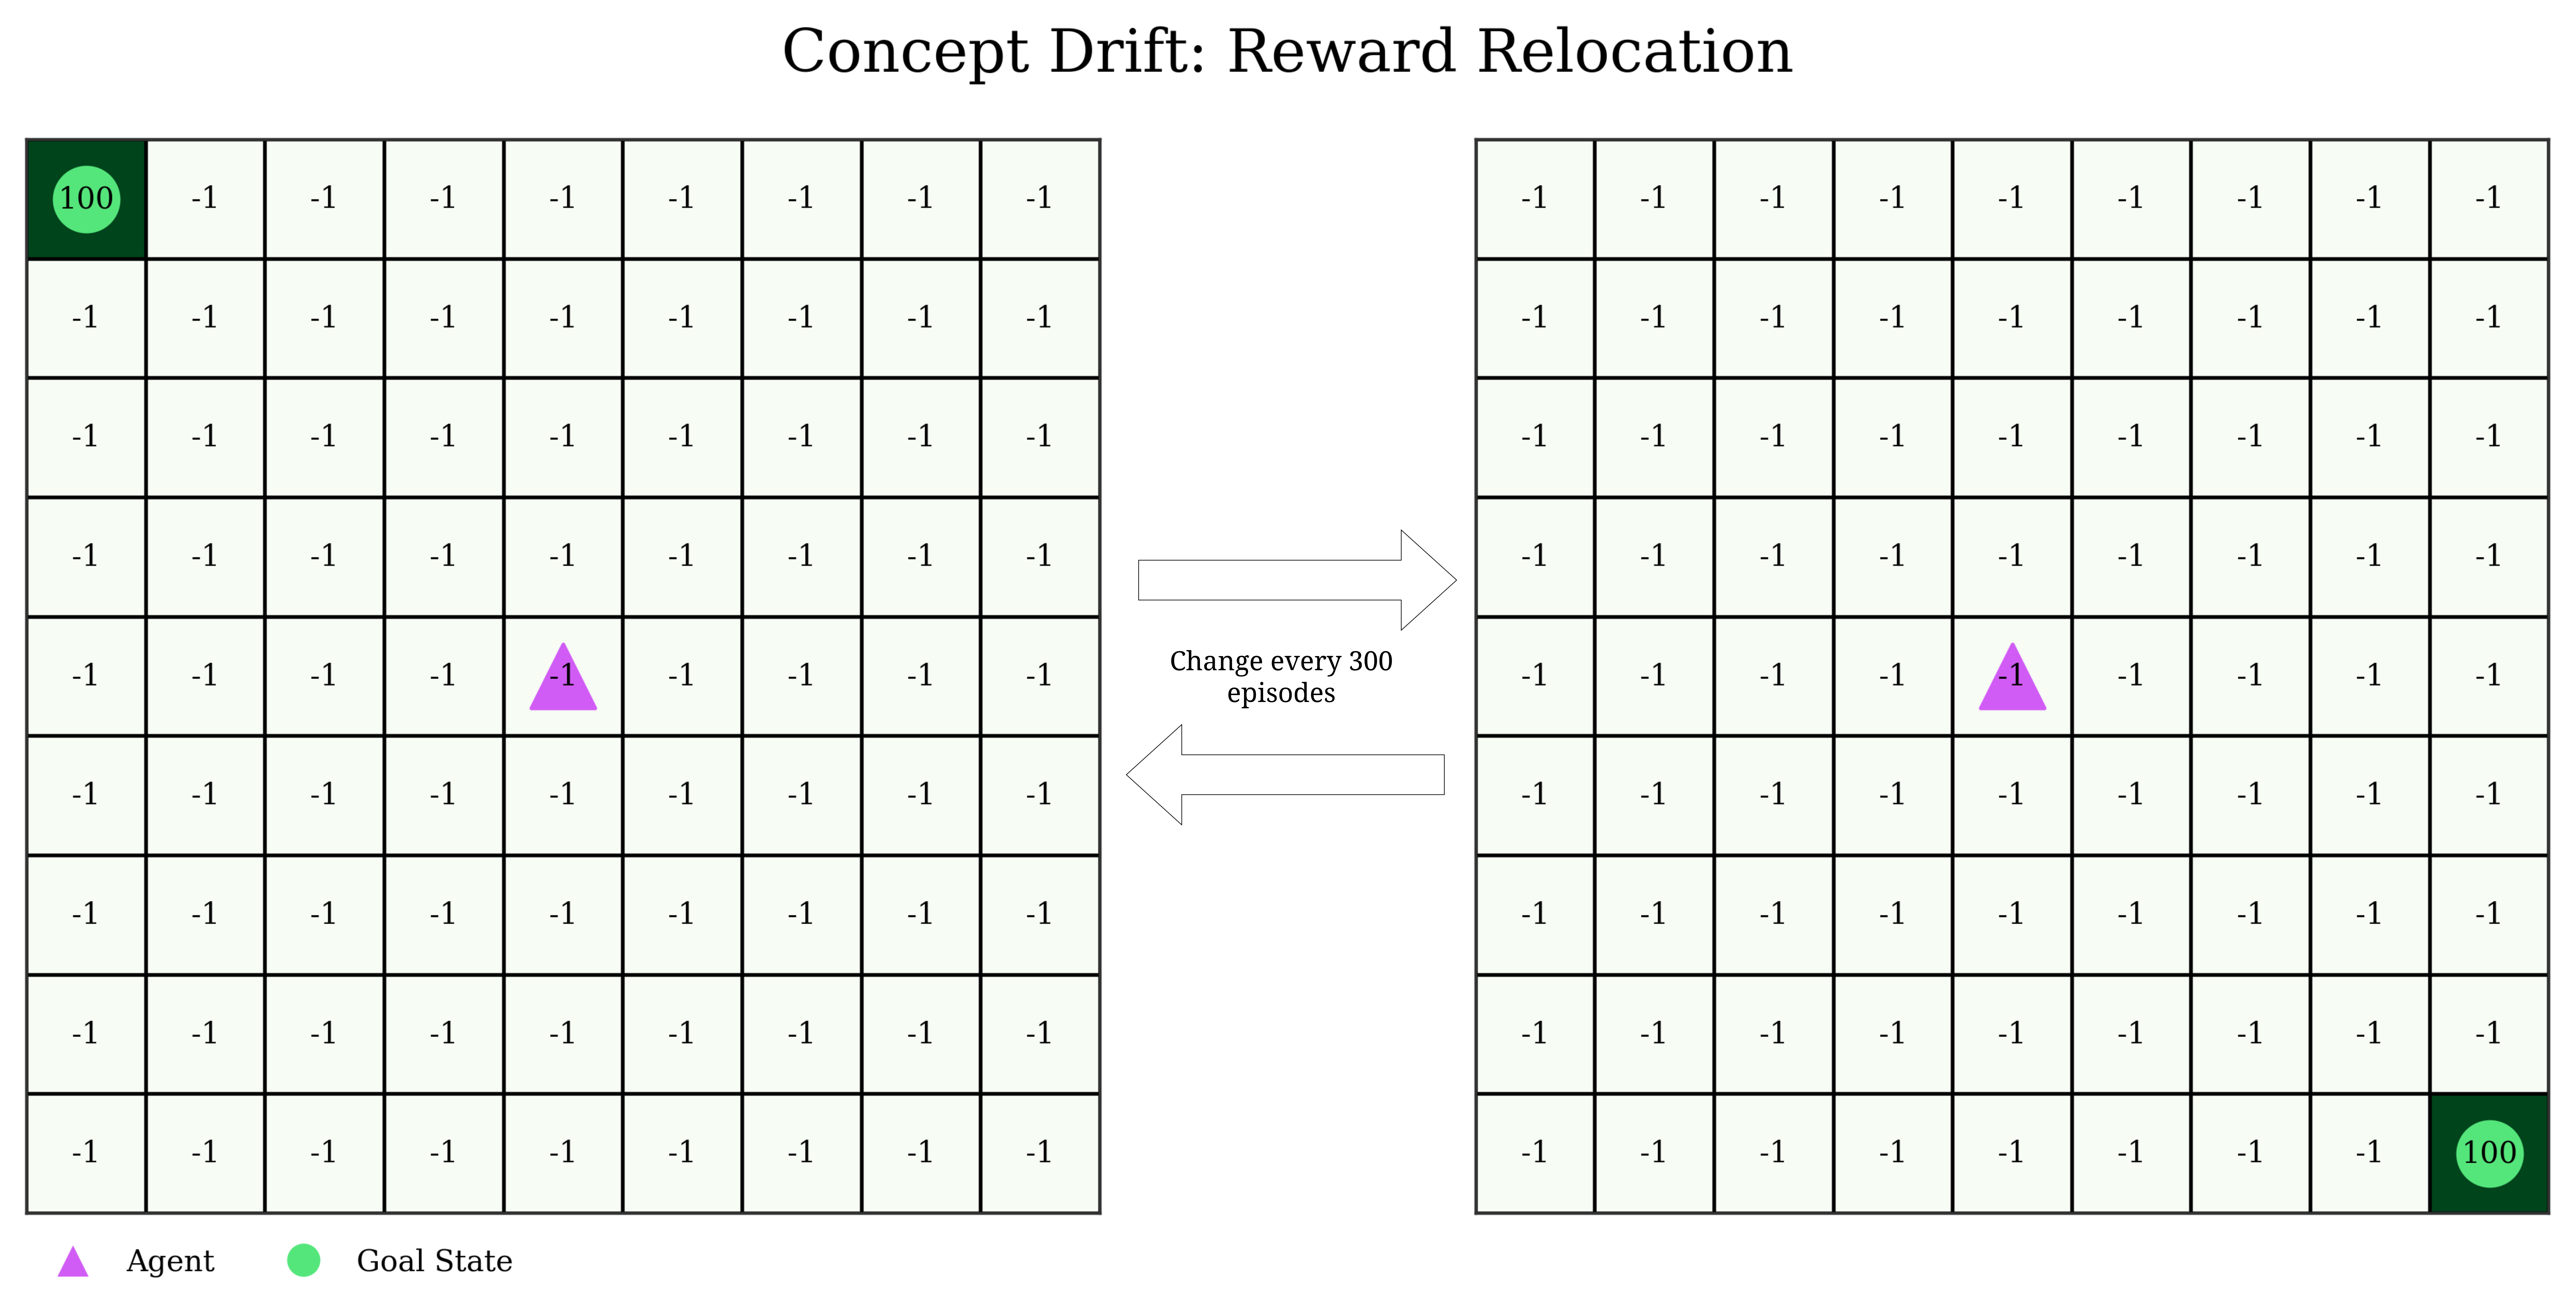
\includegraphics[width=0.9\textwidth]{figures/rewards_change}
    \caption{Non-Stationary Gridworld: Concept drift is induced by relocating the reward. The agent starts at the center and must reach the goal, which alternates between the top-left and bottom-right corners every 300 episodes.}
    \label{fig:r-change}
\end{figure*}

\endinput


% $Id: conclusion.tex 
% !TEX root = main.tex

%%
\section{\ac{RL} Agents with Adaptive Behavior}
\label{sec:implementation}

This section introduces \adaptiverl, our proposed approach for enabling \ac{RL} agents to dynamically 
adapt their behavior in response to evolving environmental conditions; specifically changes to 
environment goals and changes to agents' actions. Our method allows agents to pursue changing 
objectives throughout their operational lifespan and acquire new capabilities as tasks change over 
time. \adaptiverl is made of three main parts:
\begin{enumerate*}[label=(\arabic*)]
\item monitoring the environment for changes,
\item adapting to new goals, and
\item acquiring new behavior.
\end{enumerate*}
The implementation of our work is publicly available\footnote{Available at: \url{https://github.com/rulas99/rl_uniandes}}.

The conceptual foundation of \adaptiverl aligns with the ideas proposed 
by~\citet{abel2023definitioncontinualreinforcementlearning} for \ac{CRL}, emphasizing continual 
adaptation rather than convergence to a fixed solution. We extend tabular Q-learning by integrating 
adaptive mechanisms that enable agents to dynamically adjust their learning strategies in response 
to detected environmental changes. Similar to the approach described 
by~\citet{norman2024firstexploreexploitmetalearningsolve}, every time a change is detected, be that 
a significant change in the rewards or the introduction of new actions, our agent thoroughly explores 
the environment while retaining information of previously learned policies. The exploration process 
continues until a new policy stabilizes, to then exploit the acquired knowledge. Applying such strategy 
agents can rapidly convergence to new environment configurations, without entirely discarding 
previously learned knowledge.

To enable agents to adapt their behavior to new conditions, we introduce an adaptive mechanisms 
that adjust the agent's learning rate (\lrate{\alpha}) and exploration rate ($\varepsilon$) in conjunction 
with a concept drift detection strategy. By continuously monitoring and responding to changes in the 
environment, agents can autonomously modify their learning process at run time, enabling them 
to learn new behavior to attain their goals, even if these change. This capability positions our approach 
within the class of self-adaptive systems (SAS)~\cite{sasreview}, ensuring continual adaptation and 
resilience in non-stationary contexts.

The key to our approach is given by dynamically adjusting the learning rate (\lrate{\alpha}) based on 
the Temporal Difference (TD) error defined in \fref{eq:td_error}.

\begin{equation} \label{eq:td_error}
    TD_{error} = r_{t+1} + \gamma \cdot \underset{a}{\max} Q(s_{t+1}, a) - Q(s_t, a_t)
\end{equation}

The TD error quantifies the difference between the agent's predicted reward and the actual reward 
received. The dynamic learning rate (\lrate{\alpha^*}) is then adjusted based on the TD error following  
\fref{eq:dynamic_learning_rate}.

\begin{equation}
    \label{eq:dynamic_learning_rate}
    \alpha^* = \alpha + (\alpha_{\max}-\alpha) \cdot \frac{1}{1 + e^{-(|TD_{error}|-k)}}
\end{equation}

In the equation, \lrate{\alpha} corresponds to the base learning rate (e.g., 0.1), and $\alpha_{\max}$ is its upper bound (\eg 0.99). The parameter $k$ controls the sensitivity of the learning rate to the TD error, with higher values resulting in reduced sensitivity; thus, $k$ must be carefully tuned according to the specific characteristics of the environment and learning context. High TD errors induce a larger learning rate, enabling faster updates during exploration, whereas lower TD errors yield a more stable and conservative learning process during exploitation phases. \fref{fig:alpha} illustrates the behavior of the dynamic learning rate (\lrate{\alpha^*}) in \fref{sec:experiments} presenting the non-stationary Gridworld experiments. 

\begin{figure*}
    \centering
    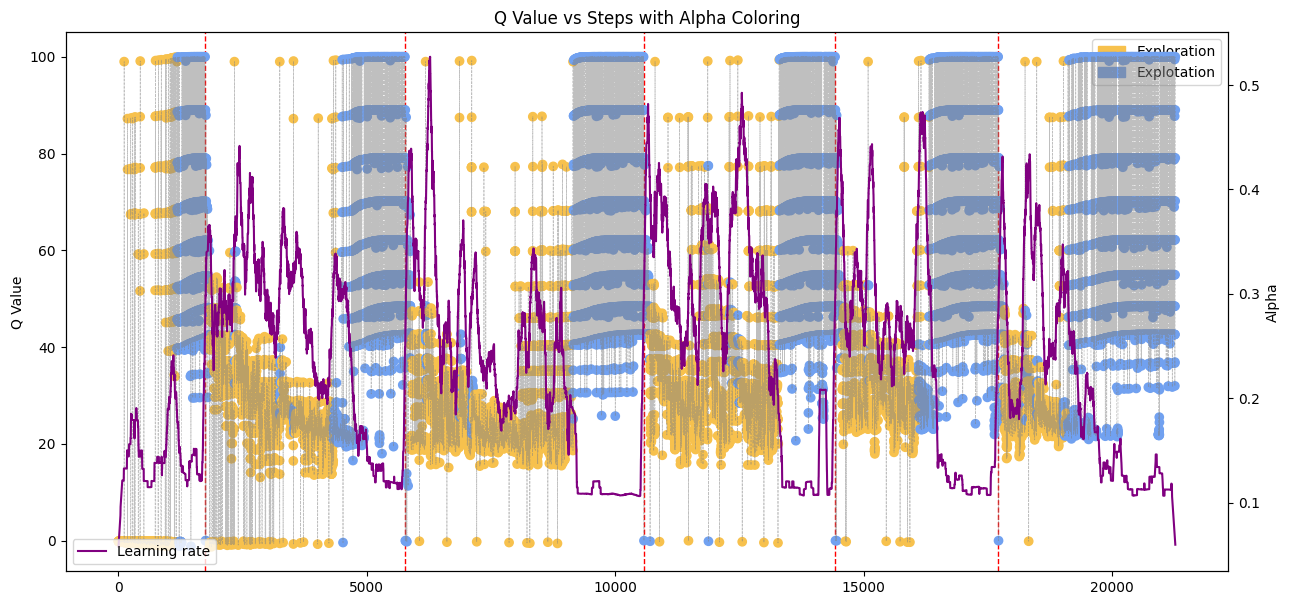
\includegraphics[width=\textwidth]{figures/alpha.png}
    \caption{\adaptiverl's adaptive behavior of the dynamic learning rate ($\alpha^*$) in Non-Stationary Gridworld experiments. Notice how $\alpha^*$ increases during exploration phases (when the TD error is high) and decreases during exploitation phases (when the TD error is low), enabling rapid convergence during exploration and stable learning during exploitation.}
    \label{fig:alpha}
\end{figure*}

%%%%
\subsection{Environment monitoring and drift detection}

The first step for agents to adapt their behavior to an evolving environment is to continuously monitor 
the environment. \ac{RL} environment monitoring is intrinsic through the interaction with the 
environment, as agents continuously observed rewards after each action execution. To detect 
changes in the environment, \ie drift, we implement the 
PH-test~\cite{mignon2017adaptive,networkdynamicrl}. The PH-test calculates the cumulative 
difference between observed rewards and the running mean reward, incorporating a sensitivity 
parameter ($\delta$). A concept drift (environmental change) is flagged when the cumulative 
difference surpasses a predefined threshold. Selecting an appropriate threshold value is crucial, as it 
determines the sensitivity of drift detection. Higher thresholds result in more conservative detection, 
while lower thresholds increase sensitivity to changes, this value must be selected based on the 
magnitude order of rewards and posible changes over them.

Building on the concept of drift detection, and following the ideas of~\citet{mignon2017adaptive}, we 
adaptively increase the exploration rate ($\varepsilon$) whenever the PH-test detects a concept drift. 
This approach promotes exploration immediately following environmental changes, enabling the agent 
to acquire new knowledge by temporarily adopting an exploration-focused policy. To ensure adequate 
exploration, the agent maintains an elevated exploration rate until rewards stabilize (\ie the cumulative 
difference is below the threshold, and  no further drifts are detected). Once stable, the exploration rate 
$\varepsilon$ uses a decay policy, leading the agent to exploit its behavior.

This adaptive drift detection mechanism ensures the agent maintains an effective balance between 
exploring new environment dynamics and leveraging previously acquired knowledge. It is crucial to 
ensure a high exploration rate after concept drift is detected consistently, so the agent can learn a 
new policy (\ie behavior) without forgetting previously acquired knowledge. \fref{fig:dynamic-eps}, 
shows the behavior of the dynamic exploration rate ($\varepsilon^*$) in our non-stationary Gridworld 
running example.

\begin{figure*}
    \centering
    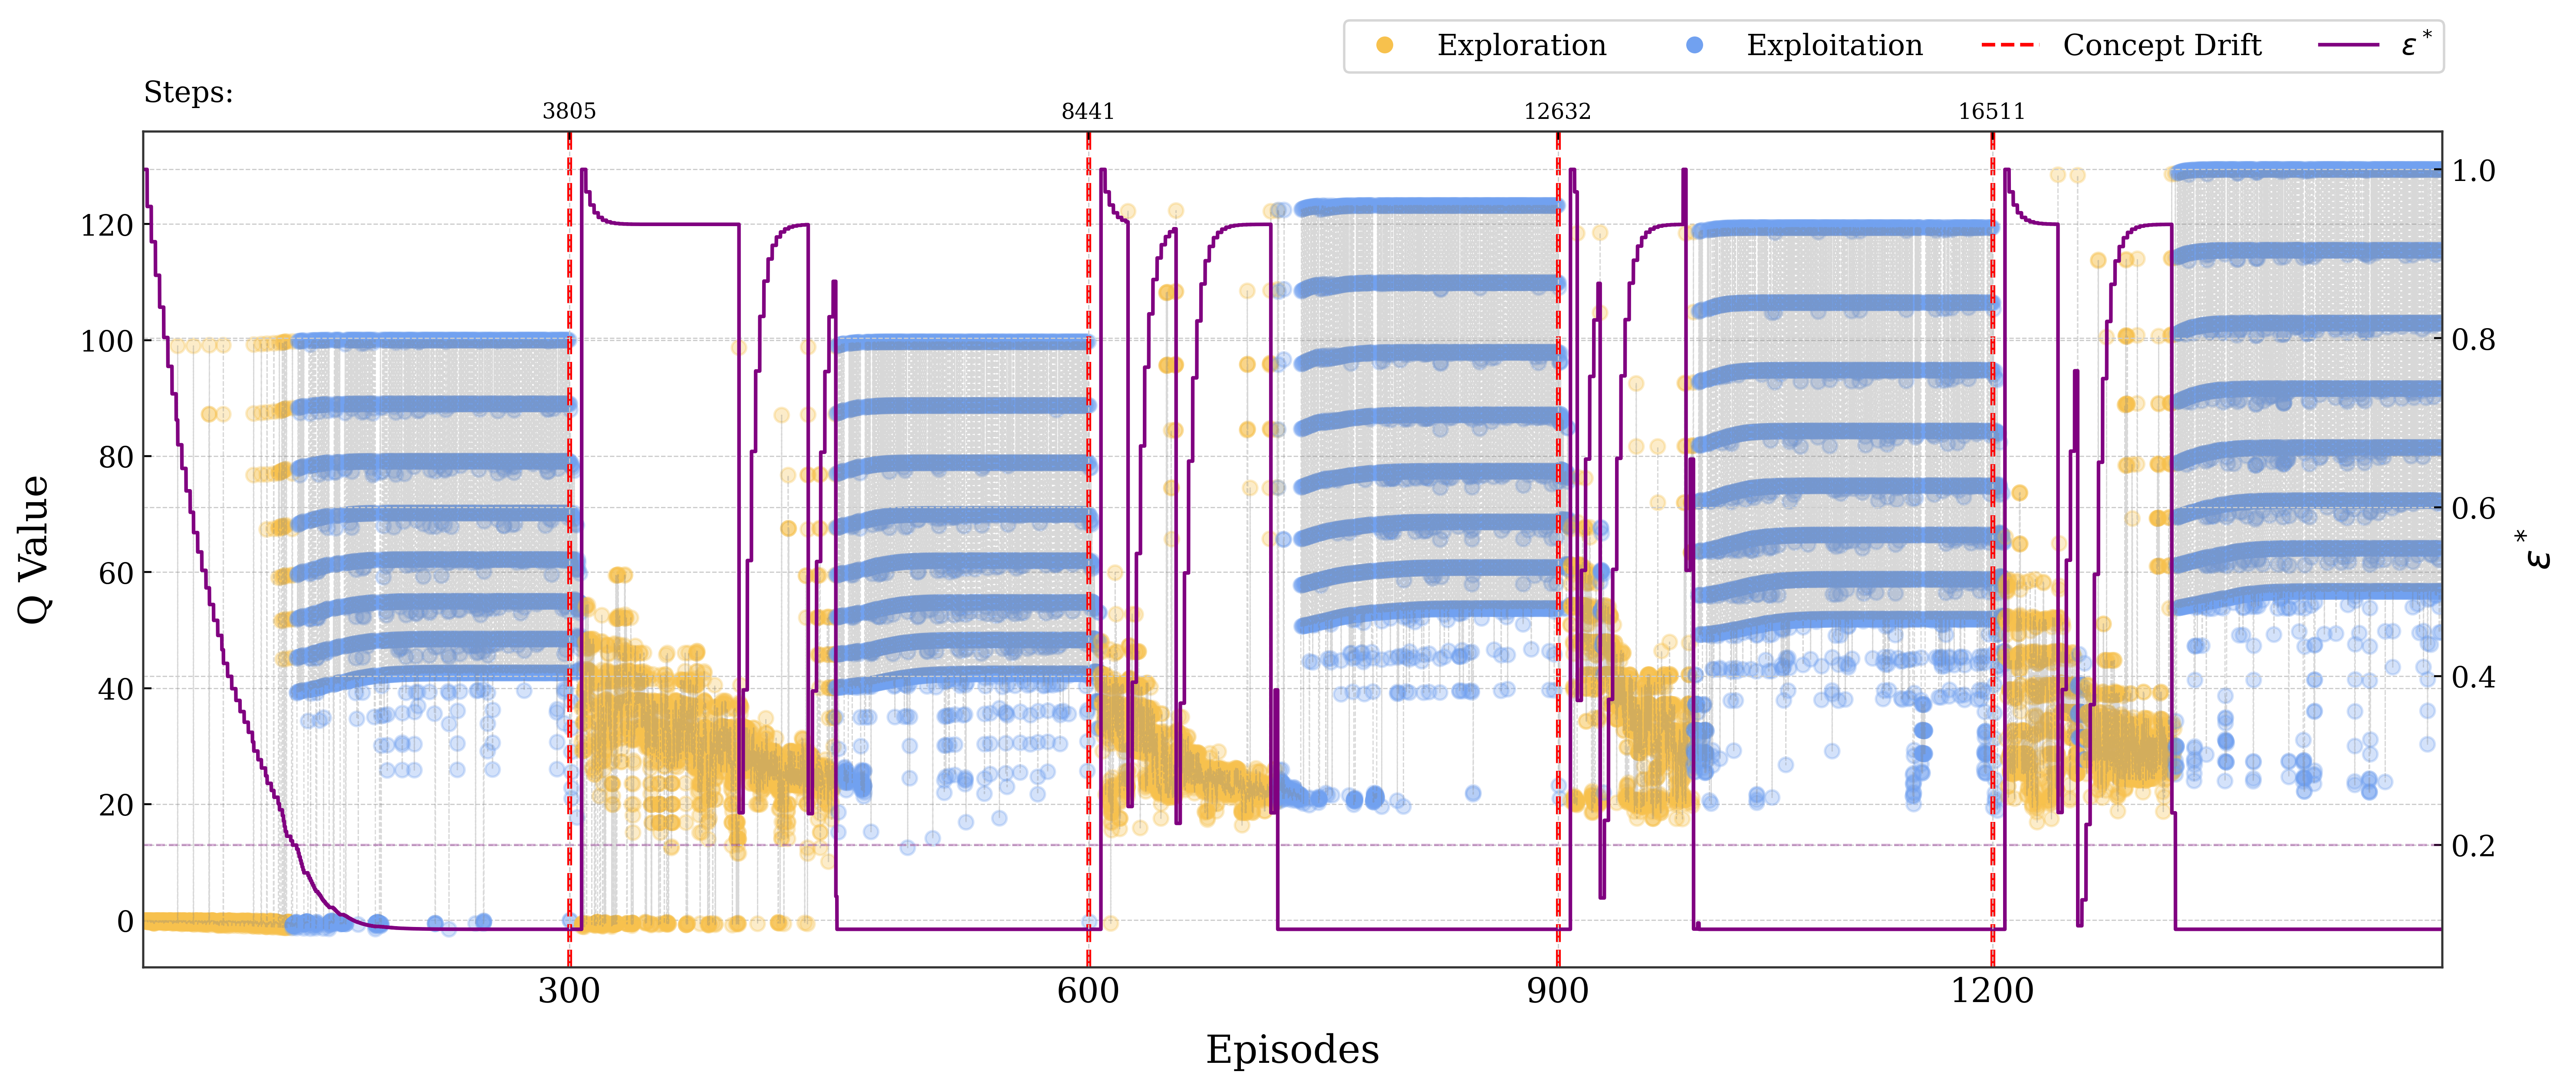
\includegraphics[width=\textwidth]{figures/eps}
    \caption{\adaptiverl's adaptive behavior of the dynamic exploration rate ($\varepsilon^*$) in Non-Stationary Gridworld experiments. Observe how $\varepsilon^*$ increases whenever a concept drift is detected by the PH-test and remains elevated until the agent consistently achieves the expected rewards (i.e., no further drift and stable rewards). Once stability is reached, $\varepsilon^*$ decays toward its minimum value, allowing the agent to exploit the acquired knowledge.}
    \label{fig:dynamic-eps}
\end{figure*}

%%%%
\subsection{Agent Adaptation to Changing Goals}
\label{sec:experiments}

To evaluate \adaptiverl's ability to adapt to environmental changes induced by a non-stationary reward function, and to compare its performance against traditional Q-learning, Gridworld. 

We compare two agents over 1,000 independent runs:  
\begin{itemize}
  \item A \emph{Standard Q-learning} agent, with fixed learning rate $\alpha=0.1$ and a fixed exponential decay for the exploration rate.
  \item A \emph{\adaptiverl} agent, employing the adaptive learning-rate and exploration-rate mechanisms described in above.
\end{itemize}
We measure (1) the number of episodes required to re-converge after each reward change, and (2) the total number of steps across all 1,500 episodes. \fref{tab:multi} reports the mean and standard deviation of the steps-to-goal for each drift, as well as the overall steps.  

\begin{table*}
    \centering
    \caption{Performance of each agent over 1,000 runs: average number of steps $\pm$ relative standard deviation (as a percentage of the mean) to reach the goal after each drift, and total steps for all 1,500 episodes (fewer steps indicate better performance).}
    \resizebox{1.01\columnwidth}{!}{
\begin{tabular}{l | c | c | c | c | c }
\toprule
\textbf{Agent} & \textbf{1st Change} & \textbf{2nd Change} & \textbf{3rd Change} & \textbf{4th Change} & \textbf{Total Steps} \\
\midrule
\adaptiverl & 135.81 $\pm$ 12.64 (9.31\%) & 475.17 $\pm$ 27.54 (5.80\%) & 767.81 $\pm$ 24.05 (3.13\%) & 1069.74 $\pm$ 26.25 (2.45\%) & 23292.07 $\pm$ 1474.13 (6.33\%) \\
Q-Learning  & 256.40 $\pm$ 11.15 (4.35\%) & -- & -- & -- & 40683.74 $\pm$ 539.44 (1.33\%) \\
\bottomrule
\end{tabular}
}

    \label{tab:multi}
\end{table*}

\adaptiverl outperforms the standard Q-learning agent on every metric. Figures~\ref{fig:alpha} and~\ref{fig:dynamic-eps} show how \adaptiverl's adaptive mechanisms enable rapid re-learning of the new goal location without erasing knowledge of previous configurations. This behavior addresses the challenge of overlapping contradictory subtasks~\cite{Bagus2022}, where identical state-action pairs may yield different rewards.

By contrast, the standard Q-learning agent converges reliably only to the first goal configuration. Figure~\ref{fig:static-eps} depicts its exploration rate decay: after each drift, the agent continues to exploit the old policy for an extended period, effectively “forgetting” previous knowledge before it begins learning the new goal location.

\begin{figure*}
    \centering
    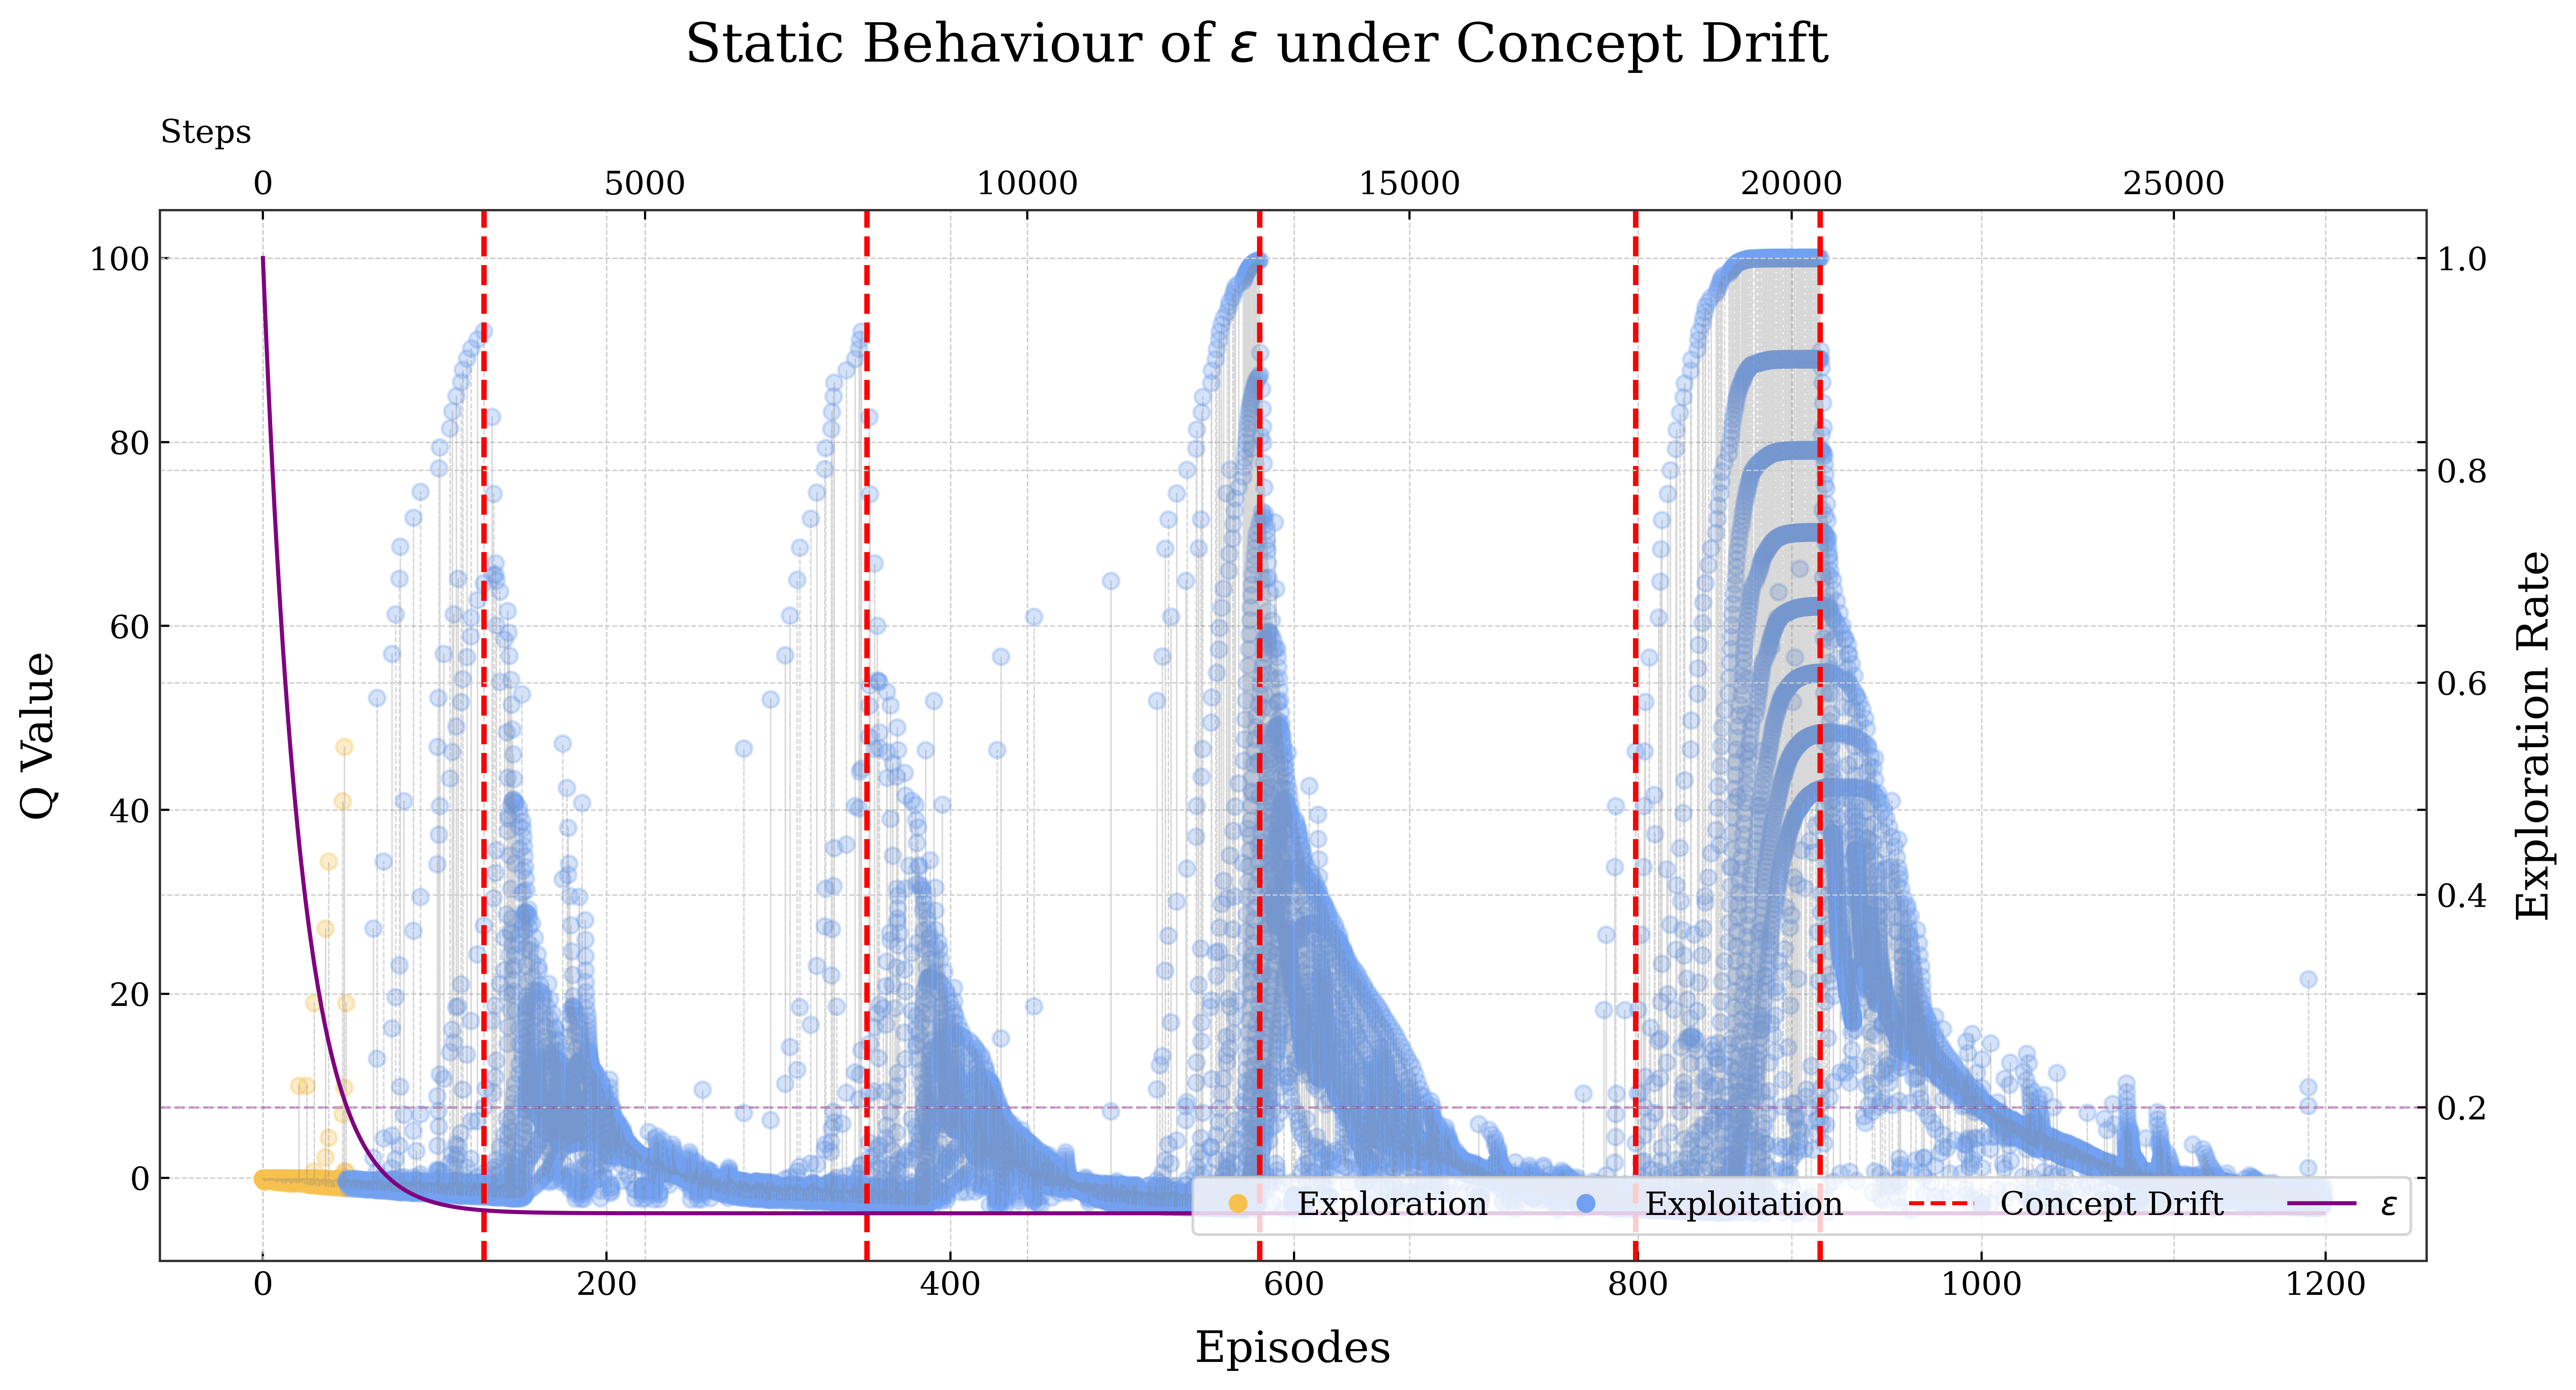
\includegraphics[width=\textwidth]{figures/trad_eps.png}
    \caption{Behavior of the static exploration rate decay ($\varepsilon$) under traditional Q-learning: the agent fails to adapt to any subsequent goal relocation, exhibiting prolonged exploitation of the obsolete policy.}
    \label{fig:static-eps}
\end{figure*}

These results demonstrate that \adaptiverl consistently outperforms standard Q-learning in adapting to changing goals and acquiring new policies without forgetting previously learned knowledge. As shown in Figure~\ref{fig:q-value-comp}, after 1,500 episodes, \adaptiverl maintains high Q-values for all previous goal configurations, whereas traditional Q-learning must overwrite its Q-values each time the goal relocates. Notably, \adaptiverl preserves prior knowledge by promoting exploration for a sufficient period after each detected drift and by scaling updates according to the TD-error magnitude. This approach not only prevents catastrophic forgetting but also enables the agent to handle both contradictory and non-contradictory overlapping subtasks---such as when goals are randomly sampled in nearby regions rather than at the exact same cell\footnote{Animated simulations of these and other scenarios are available at: \url{https://github.com/rulas99/rl_uniandes/tree/main/simulations}}.

While \adaptiverl introduces modest overhead due to drift detection and adaptive updates, its overall 
run-time is actually lower. Using our experimental setting $1,000$ runs take approximately 5
minutes for \adaptiverl, while it takes around 8 minutes to complete all runs with the baseline Q-learning implementation. This efficiency gain results directly from the reduced number of steps needed to reach the goal after each drift. Specifically, \adaptiverl converges in significantly fewer steps than the standard agent---requiring about 1.9x fewer iterations after the first drift and 1.7x fewer over the full 1,500 episodes---highlighting the practical advantages of our adaptive mechanisms in dynamic environments.

\begin{figure*}
    \centering
    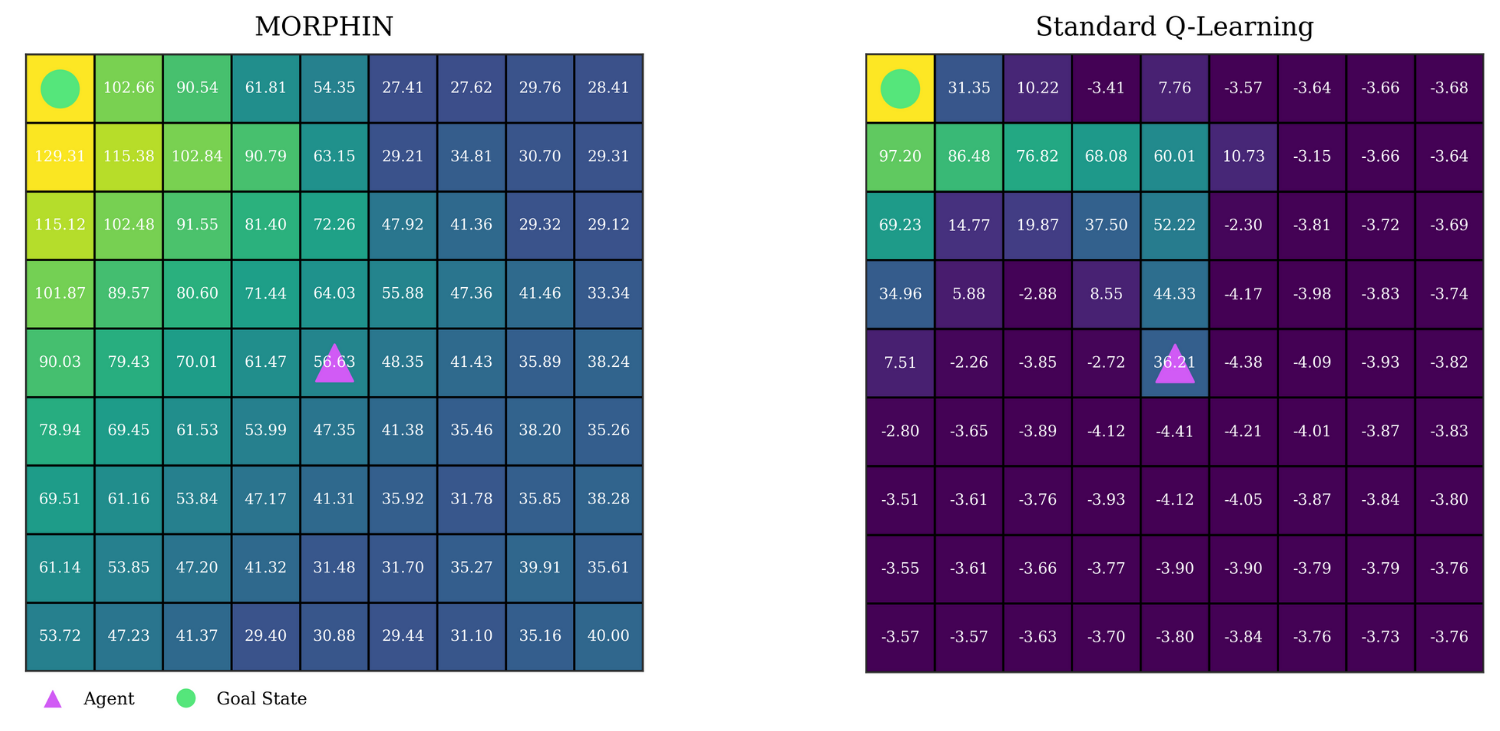
\includegraphics[width=\textwidth]{figures/q_map_comp}
    \caption{Comparison of Q-value heatmaps after 1,500 episodes in a Non-Stationary Reward Environment: (left) \adaptiverl preserves high Q-values across alternating goal configurations; (right) Standard Q-learning must overwrite past knowledge to learn each new goal.}
    \label{fig:q-value-comp}
\end{figure*}

%%%%
\subsection{Acquisition of new actions}
In the next Section~\ref{sec:validation}, we present a real-world use case for traffic light control, where the agent is provided with a new set of actions following concept drift detection. This enables the agent to efficiently learn how to utilize the new actions and optimize traffic flow by adapting its policy to varying congestion levels. The agent can acquire new capabilities without forgetting previously learned behaviors, maintaining adaptability to changing environmental conditions.

These adaptive mechanisms equip the agent to effectively manage learning under varying and unpredictable conditions, enabling continuous adaptation and efficient knowledge transfer between different environmental states. The concept drift detection method with the dynamic exploration rate allows the agent to rapidly respond to new information without discarding previously learned knowledge, achieving a greater resilience and performance stability over its lifespan. 


\endinput


% $Id: conclusion.tex 
% !TEX root = main.tex

%%
\section{Validation}
\label{sec:validation}

This section evaluates \adaptiverl in a realistic traffic-signal control scenario under non-stationary congestion. Intelligent traffic management is a canonical application of self-adaptive systems~\cite{HENRICHS2022106940}, and recent meta-\ac{RL} work has shown benefits when reward functions change with traffic saturation~\cite{meta-rl-traffic}. Here, we model two crossing lanes (C1 vertical, C2 horizontal) with Poisson arrivals and dynamically switch congestion levels (changing $\lambda$ parameter) to induce concept drift.  

\subsection{Traffic Environment}
We implement a custom \texttt{TrafficEnv} (exending OpenAI's Gym library~\cite{towers2024gymnasiumstandardinterfacereinforcement}) whose state is $(c_1,c_2)$, the number of queued vehicles on lanes C1 and C2 (each in $[0,\mathit{max\_state}]$). At each time step the agent selects one of three signal phases:
\[
\actions={\,(5,2),\;(2,5),\;(3,3)\}
\]
indicating service capacities (percentage of the lane cleared per step) for C1 and C2, respectivily. During each step, service is applied to C1, new vehicles arrive to C2 (Poisson with rate $\lambda_{2}$), then service is applied to C2, followed by arrivals to C1 (Poisson with rate $\lambda_{1}$). Any unused service capacity incurs a penalty:
\[
\mathrm{penalty} \;=\; 3\times(\text{waste}_{C1} + \text{waste}_{C2})\,,
\]
discouraging “over-serving” when queues are small.

The \emph{dynamic reward} combines congestion cost and service penalty:
\[
r = 
\begin{cases}
-(2c_1 + c_2)\quad &\text{if }c_1>7 \;\wedge\;c_1>c_2,\\
-(c_1 + 2c_2)\quad &\text{if }c_2>7 \;\wedge\;c_2>c_1,\\
-(c_1 + c_2)\quad &\text{otherwise}
\end{cases}
\;-\;\mathrm{penalty}\,
\]
Episodes last 30 steps. We induce two concept drifts by changing arrival rates at episodes 3,000 and 8,000 for a total run of 10,000 episodes:
\[
(\lambda_1,\lambda_2):
\;(4,2)\;\to\;(5,7)\;\to\;(3,1)
\]

We compare:
\begin{itemize}
  \item A \emph{standard Q-learning} agent with fixed $\alpha=0.1$, and $\varepsilon$ decayed exponentially to $0.01$.
  \item An \emph{\adaptiverl} agent that uses the PH-test to detect drifts in episode-rewards, resets $\varepsilon\!=\!1$ upon detection, and adaptively adjusts $\alpha$ based on the TD-error (cf.\ Section~\ref{sec:implementation}).  When a drift is detected, it also \emph{appends} two new phases:
  \[
    (7,3)\quad\text{and}\quad(3,7),
  \]
  allowing finer control under high congestion. Old actions are never removed.
\end{itemize}

\subsection{Results}
Figure~\ref{fig:traffic-learning-curve} plots the cumulative mean reward (over the last 500 episodes) for both agents. The green vertical line marks the PH-test detection at episode 3004; the second drift at episode 8000 was not flagged, since the new arrival rates produce a reward distribution within the original sensitivity threshold.

\begin{figure*}
    \centering
    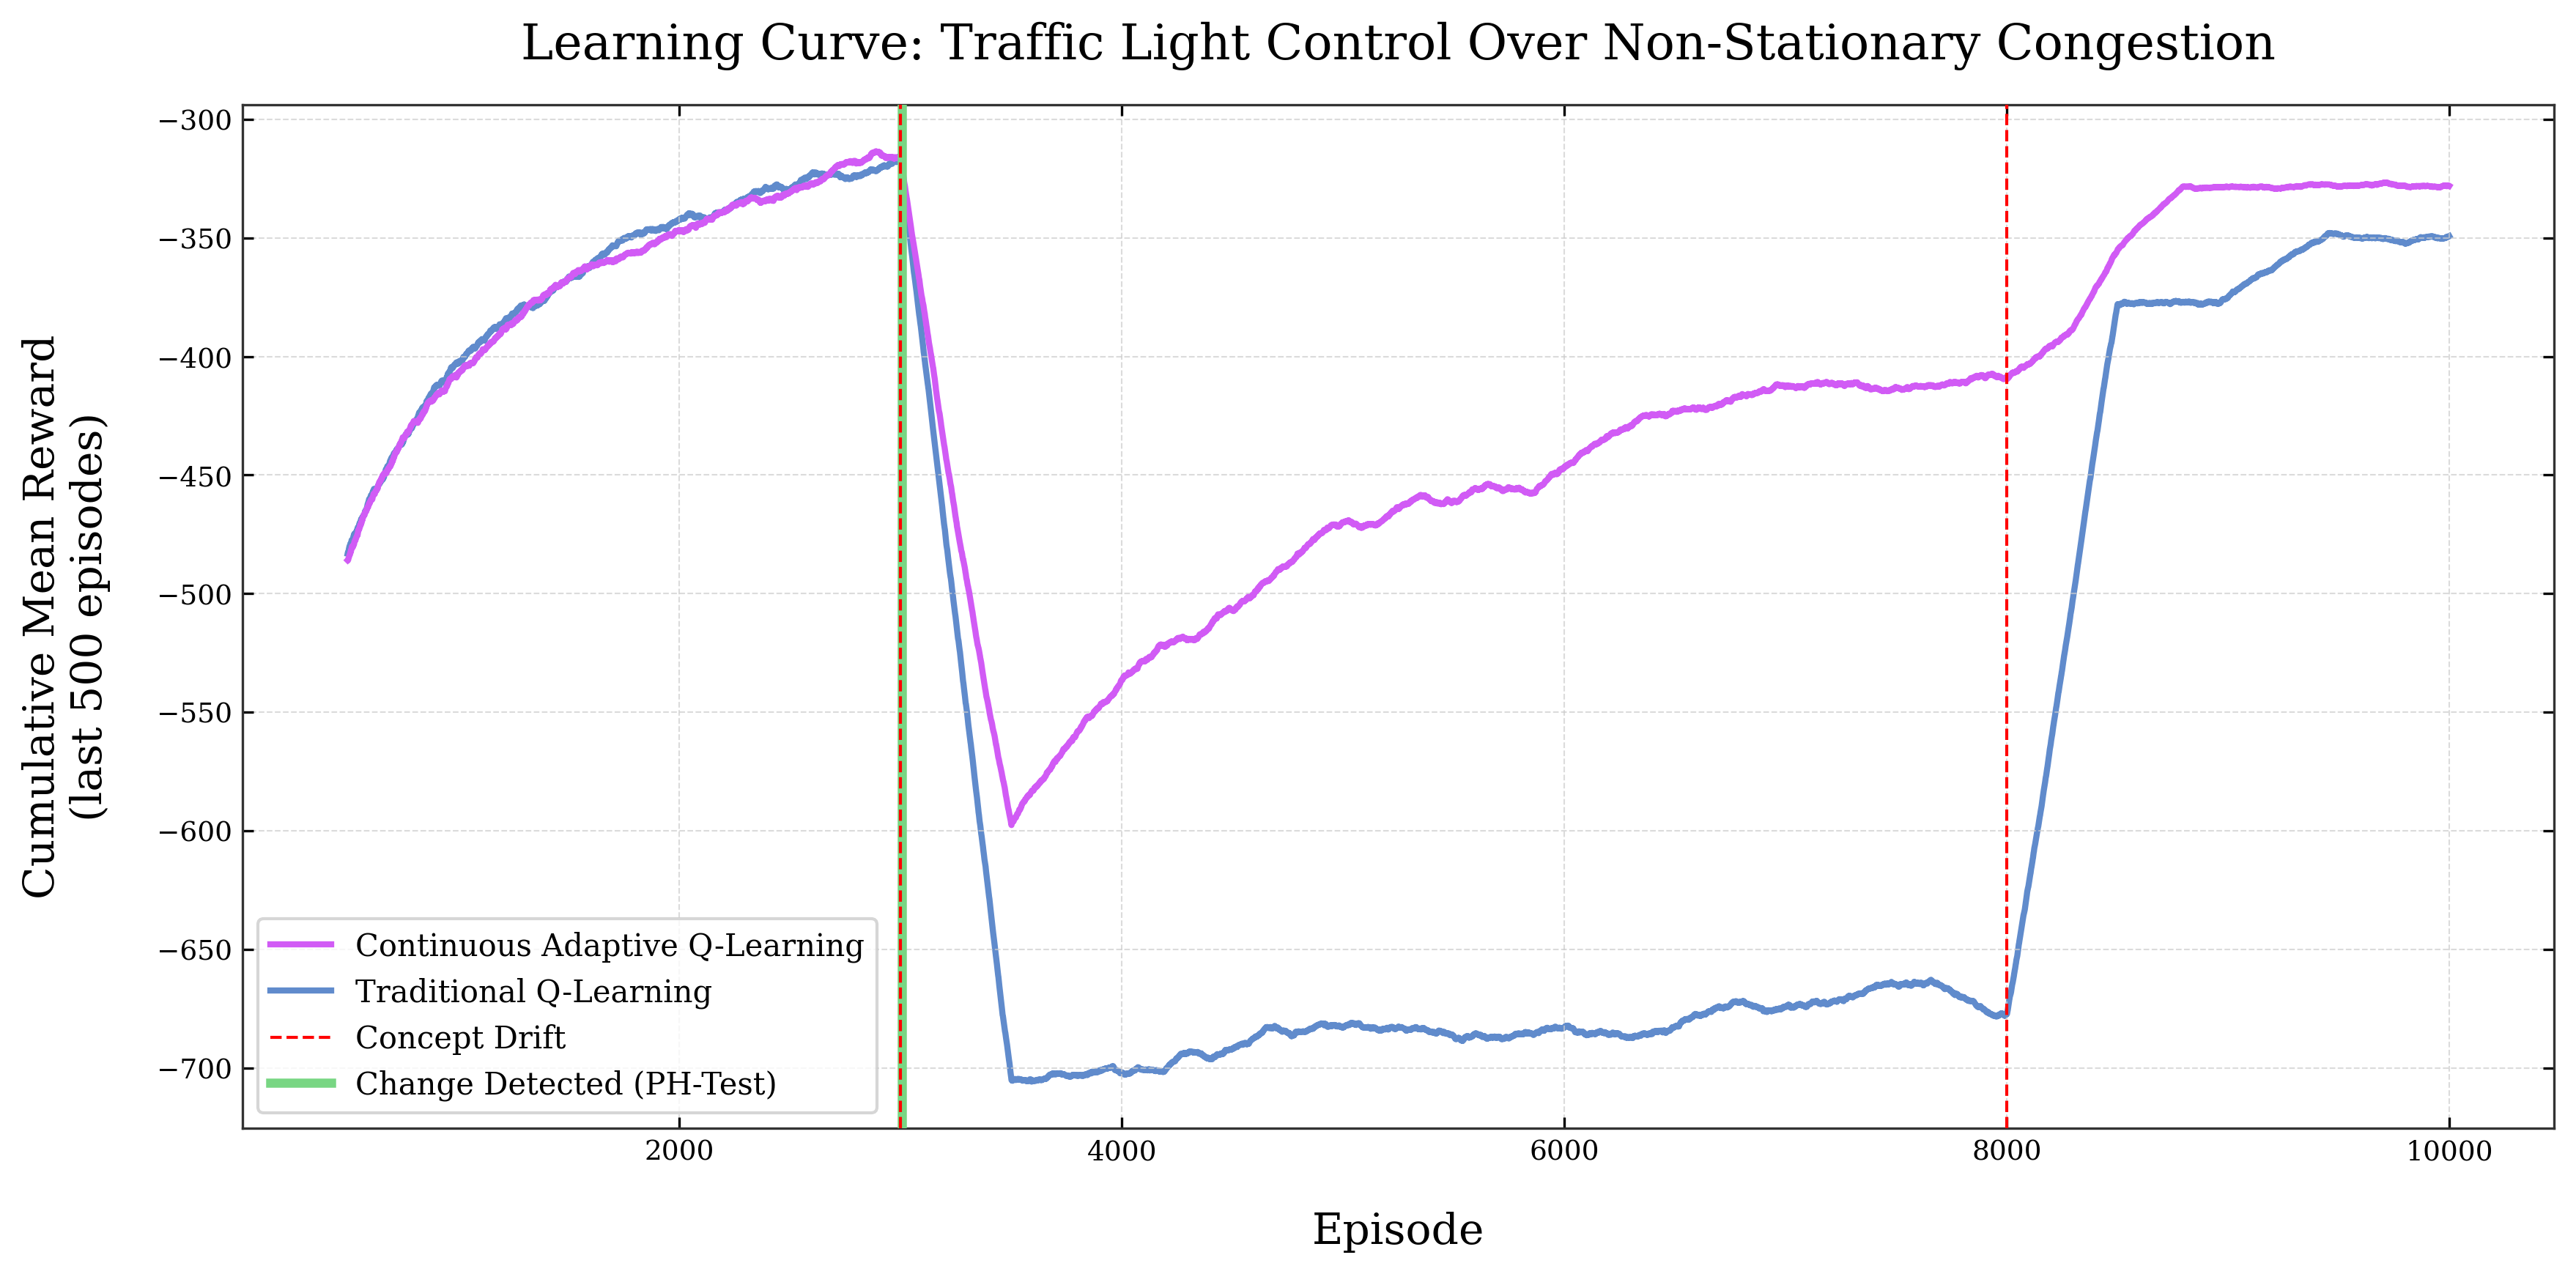
\includegraphics[width=\textwidth]{figures/traffic_learning_curve.png}
    \caption{Learning curves for traffic-signal control under non-stationary congestion. Rapidly recovers after the first drift thanks to extension of action set after PH-Test detection, while traditional Q-learning suffers prolonged performance drops.}
    \label{fig:traffic-learning-curve}
\end{figure*}

Initially, both agents improve steadily. After the first drift, \adaptiverl promptly increases exploration, exploits its new actions $(7,3)$ and $(3,7)$, and regains performance within a few hundred episodes. In contrast, the standard agent endures a deep, slow recovery. The built-in penalty for wasted green time ensures \adaptiverl does not “over-serve” when queues shrink, automatically balancing old and new phases without discarding any actions.

This traffic-signal case confirms that \adaptiverl can:
\begin{enumerate}
  \item Detect and react to non-stationary congestion via the PH-test, boosting exploration exactly when needed and the adaptive mechanisms that distinguish \adaptiverl.
  \item Seamlessly incorporate new signal phases---analogous to real-world reprogramming of traffic lights---without removing prior options.
  \item Leverage a dynamic reward (with penalization) to avoid excessive service when traffic is light, resulting in resource-efficient policies.
\end{enumerate}
In practice, modern traffic controllers can update phase timings in real time; endowing them with self-adaptive intelligence, as in \adaptiverl, allows continuous, automated adjustment to changing traffic patterns without manual retuning.

\endinput


% $Id: conclusion.tex 
% !TEX root = main.tex

%%
\section{Related Work}
\label{sec:related}

\ac{RL} inherently deals with the critical trade-off between exploration and exploitation, which 
significantly influences the performance of the learned policy. An agent must explore sufficiently to 
avoid settling for suboptimal solutions, yet excessive exploration can lead to inefficient training. 
Hence, determining an optimal balance between these two strategies is crucial for achieving 
high-quality solutions~\cite{sutton98}.

Many adaptive strategies have been proposed to manage this balance dynamically.~\citet{tokic2010} 
and~\citet{mignon2017adaptive} introduce adaptive implementations of the classic 
$\varepsilon$-greedy policy, highlighting the effectiveness of dynamically adjusting $\varepsilon$ values 
rather than maintaining them statically.~\citet{mignon2017adaptive} demonstrate how an adaptive 
approach enhances performance in both stationary and non-stationary environments by employing 
the Page-Hinkley Test (PH-test) for detecting environmental concept drifts.

Building on the exploration-exploitation dilemma, \citet{norman2024firstexploreexploitmetalearningsolve} 
propose First-Explore, a meta-\ac{RL} approach utilizing distinct policies dedicated to exploration 
and exploitation. Unlike conventional methods that directly optimize cumulative rewards, First-Explore 
trains these two separate policies and later combines them to form an inference policy that strategically 
explores initially for $k$ episodes, sacrificing immediate rewards for greater cumulative future gains. 
This strategy specifically addresses the limitations faced by existing methods that tend to prematurely 
converge to suboptimal solutions due to inadequate early exploration.

Hyperparameter optimization, particularly the learning rate, also plays a crucial role in training 
effective \ac{RL} models. A well-known example is the Adam 
optimizer~\cite{kingma2017adammethodstochasticoptimization}, which dynamically adjusts the learning 
rate based on past gradient information to facilitate more efficient training convergence. Extending 
this line of research, \citet{dynamicrlalpha} propose a dynamic learning rate approach tailored for deep 
\ac{RL} scenarios. Their method adaptively selects optimal learning rates at different training stages, 
demonstrating substantial performance improvements by considering the non-stationarity inherent to 
\ac{RL} tasks.

Transfer learning strategies, like the Transferred Q-Learning~\cite{chen2022transferredqlearning}, 
have demonstrated improvements in convergence rates. By reusing previous knowledge from similar 
tasks, showing that these methods effectively accelerate the learning process.

The methods mentioned above—focused on the adaptivity of learning parameters and the reuse of prior knowledge—closely align with the concept of \ac{CRL}~\cite{khetarpal2022continualreinforcementlearningreview}.
\citet{abel2023definitioncontinualreinforcementlearning} define \ac{CRL} as a setting in which “the best agents never stop learning,” contrasting this with traditional \ac{RL}, which typically treats learning as the identification of a static solution rather than a process of continuous adaptation.
Recent work has begun to explore \ac{CRL} specifically through the lens of Q-learning.
\citet{Bagus2022} provide one of the first systematic empirical studies of \textbf{Continual} Q-learning, using a decomposition of the original task into overlapping but non-contradictory sub-tasks to evaluate the effectiveness of continual learning mechanisms.
Another approach for Continual Q-Learning comes from \citet{araujo2020controladaptiveqlearning}, who propose Adaptive Q-Learning (AQL) and its single-partition variants SPAQL and SPAQL-TS. These algorithms dynamically refine state–action partitions during training and demonstrate strong sample efficiency in continuous control problems such as CartPole, without relying on fixed discretizations.

Various studies have shown \ac{RL} as a potent tool for self-adaptive systems in real-world 
applications~\cite{HENRICHS2022106940}. Notable examples of \ac{RL} implementations 
include the use of adaptive $\varepsilon$-greedy policies to dynamically adjust exploration-exploitation 
trade-offs for \ac{IOT} security in edge computing~\cite{iotdynamicrl}, the integration of \ac{RL} 
with active learning and concept drift detection mechanisms (like PH-Test) for network monitoring to 
effectively identify potential threats~\cite{networkdynamicrl}, or the use of \ac{RL} macro actions to 
continuously learn adaptation strategies~\cite{cardozo23}.

Our approach compares with the state-of-the-art in that \authorcomment[idea]{RD}{Complete?}


\endinput

% $Id: conclusion.tex 
% !TEX root = main.tex

%%
\section{Conclusion and Future Work}
\label{sec:conclusion}
We have demonstrated that \adaptiverl, a self-adaptive Q-learning agent, can effectively detect and respond to non-stationary environments. By leveraging concept drift detection and dynamically adjusting its learning rate and exploration parameters, \adaptiverl consistently outperforms standard Q-learning agents in scenarios where the reward function changes over time. Its adaptive mechanisms are well aligned with the principles of self-adaptive systems, enabling the agent to autonomously adjust its behavior in response to evolving environmental conditions.

\adaptiverl's adaptability is aligned with the definition proposed by~\citet{abel2023definitioncontinualreinforcementlearning}, treating learning as a continuous process rather than a one-time optimization. Notably, it addresses one of the major challenges in continual reinforcement learning (CRL): the problem of catastrophic forgetting.\adaptiverl retains prior policy knowledge while adapting to new configurations, enabling knowledge reuse and accelerating convergence—even when faced with overlapping contradictory subtasks, as highlighted by~\citet{Bagus2022}.

We further validated \adaptiverl in a realistic traffic signal control scenario, where the agent successfully adapted to changing traffic patterns and performance requirements. The use of a dynamic reward function, including penalties for over-serving, proved effective in promoting resource-efficient policies. Additionally, by appending new signal phases (i.e., new actions) upon drift detection, \adaptiverl demonstrated its ability to acquire new capabilities without discarding existing ones. This is particularly relevant in real-world traffic systems, where signal configurations can be updated in near real time; equipping them with adaptive intelligence allows for continuous optimization without the need for manual retuning.

\adaptiverl stands as a promising approach for self-adaptive systems requiring lightweight, real-time learning solutions in environments with limited computational resources.

In future work, we plan to integrate \adaptiverl with complementary mechanisms, such as active learning, and deploy it in edge devices for real-world applications (e.g., \ac{IOT}). Additionally, we aim to generalize its core principles from tabular methods to deep learning architectures. This includes incorporating memory-based plasticity to support knowledge reuse across tasks and enabling online test-time adaptation, allowing agents to respond to new situations without requiring full retraining.Finally, ...\authorcomment[idea]{RD}{Complete?}

\endinput



%\section*{Acknowledgment}

\printbibliography

\end{document}
